\chapter{Lo stato attuale}
\thispagestyle{empty}
\section{Le modifiche al giorno d'oggi}
%Parla anche dell'assenza di organi per la misurazione dei consumi (elettrici e termici) e quindi problemi per la valutazione energetica \emph{ante-operam} e per il rispetto ai requisiti \emph{CAM}.\vspace{1em}
Nel primo capitolo si sono descritti in maniera sommaria l'architettura, l'edilizia e gli impianti presenti nell'intero complesso ospedaliero (al momento della costruzione) riportando le parole dell'\tit{ing.}{Corrado Beguinot}. 

In questo capitolo, invece, si vuole dare ampio spazio alle condizioni attuali del policlinico e dell'edificio stesso, riportando i dati di input inseriti all'interno dello studio pre-riqualificazione energetica e riferiti, quindi, allo stato di fatto. 

Riferendosi alla sola centrale termica del policlinico, nel marzo del 2004 è entrato in servizio il gruppo di cogenerazione a gas metano della potenza elettrica di \n{5.5}{MW} e \n{9}{MW} di potenza termica con caldaia a recupero. Il gruppo è costituito da:
\begin{itemize}
	\item una turbina \emph{Solar Turbines} modello \emph{Taurus T60};
	\item un produttore di energia elettrica \emph{Le Roy Somer -- Emerson};
	\item una caldaia a vapore \emph{Ruths}.	
\end{itemize}
I primi due sistemi (turbina e alternatore) sono assemblati in un unico package di produzione \emph{Turbomach} con in coda la caldaia a recupero.

La centrale è corredata anche da:
\begin{itemize}
	\item \num{4} assorbitori di vapore per produzione acqua refrigerata della potenza di \n{2691}{kW} cadauno \emph{ABTF750 -- Trane};
	\item \num{1} gruppo di assorbimento \emph{McQuay} da \n{4301}{kW};
	\item \num{2} caldaie \emph{Biasi} da \n{12}{MW} cadauna da utilizzarsi sporadicamente per integrazioni (nei periodi invernali con climi rigidi) e/o sostituzione della caldaia a recupero (in caso di manutenzione/guasto del gruppo di cogenerazione).
\end{itemize}

L'acqua surriscaldata viene prodotta a \n{130}{\degreeCelsius} e non più a \n{170}{\degreeCelsius} come avveniva in passato. I reflui termici alimentano da un lato la rete di teleriscaldamento e dall'altra il gruppo di assorbitori bistadio che a loro volta servono la rete di teleraffrescamento. Dei \num{4} assorbitori uno è di back-up. Un'altra modifica che ha interessato la centrale termica è stata la sostituzione delle torri evaporative giustificata da costi di manutenzione eccessivi nonché da un'evidente usura della struttura portante in legno. 

Per quanto riguarda la stagione estiva, invece, i gruppi ad assorbimento non risultano essere in grado, nonostante la recente installazione delle nuove macchine, di coprire il fabbisogno \emph{freddo} di tutto il policlinico a causa della diffusione dei fancoil e delle batterie di raffreddamento delle UTA (più numerose oggi che in passato). E se il gruppo ad assorbimento risulta essere \emph{sottodimensionato} ai carichi presenti oggigiorno nel policlinico, vi sono comunque i reflui termici del cogeneratore/caldaia che in estate non vengono utilizzati: si perde in ambiente una grande fonte di energia ad elevata temperatura. Nell'attesa di una riqualificazione dei vari edifici a cui sarebbe seguito senz'altro il montaggio dei fancoil, molti dipartimenti si sono autogestiti utilizzando \emph{split} per migliorare le condizioni termoigrometriche dei locali nella stagione estiva. Questo ha comportato un aumento di consumo di energia elettrica in tutto il policlinico.

\section{L'edificio 2}
Tutto il corpo di fabbrica è destinato alla \emph{Cardiochirurgia}.
\begin{figure}[t]
	\centering
	\includegraphics[width=\textwidth]{6_2_cap/img/SatellitareED2}
	\caption[Veduta satellitare dell'edificio 2 e dei suoi 5 corpi]{Veduta satellitare dell'edificio 2 e dei suoi 5 corpi. Fonte: \emph{Google Earth}.}
\end{figure}

Esso è costituito da 5 edifici:
\begin{itemize}
	\item Corpo A: è l'edificio principale. Di sviluppo longitudinale lungo un asse orientato lungo la direttrice NE--SO, è costituito da 6 piani fuori terra. Contiene le degenze, gli ambulatori, l'Emodinamica al piano terra, l'UTIC (Unità di Terapia Intensiva Coronarica) al primo piano e il blocco operatorio con terapia intensiva al quinto piano. La sua superficie coperta è di \n{5610}{m^2}, per singolo piano è di \n{935}{m^2} e un volume di circa \n{18700}{m^3};
	\item Corpo B: contiene gli stabulari. Di pianta pressoché quadrata (\n{102}{m^2}) è alto solo 1 piano; 
	\item Corpo C: contiene laboratori e ambulatori. E' di pianta rettangolare e alto solo 1 piano. Estensione di \n{812}{m^2};
	\item Corpo D: contiene ambulatori, studi medici e laboratori. Di pianta quadrata (\n{217}{m^2}) è alto solo 1 piano; 
	\item Corpo E: contiene ambulatori cardiologici, geriatrici e di medicina interna, vari laboratori e studi medici. È alto solo 1 piano con un'estensione di \n{305}{m^2}.
\end{itemize}

L'edificio 2 preserva tutte le opere edili e alcune impiantistiche realizzate all'epoca della sua costruzione. Non è difficile dedurre, quindi, che allo stato attuale sia i comportamenti estivi e invernali dell'involucro come le efficienze termo-meccaniche dell'impianto idro-aeraulico siano quantomeno inferiori a quelli consigliati dalla norma attuale vigente. In \vref{pan} è presente una panoramica in cui è possibile apprezzare i vari corpi. In \vref{IFC} sono state riportate \num{3} immagini del modello tridimensionale dell'edificio 2 costruito con \textbf{IFC Builder}. Il file è stato poi importato nel \textbf{LOAD} da cui sono stati estratti i carichi termici. È interessante notare la verosimiglianza delle suddette immagini con quelle reali riportate in \vref{ed21} e \ref{ed22}.

L'analisi progettuale ha come oggetti di intervento il corpo A e C. In particolare, del primo non si interessa nel quinto piano (dove è situato il blocco operatorio) e degli impianto dell'UTIC e dell'Emodinamica.

Riassumendo: il corpo A verrà riqualificato \emph{civilmente} in tutti i piani escluso il quinto piano e i tre pozzi delle scale; l'intervento impiantistico interesserà, invece, tutto il corpo A esclusi i tre pozzi delle scale, l'UTIC, l'Emodinamica e tutto il quinto piano; il corpo C verrà riqualificato integralmente sia \emph{civilmente} che \emph{impiantisticamente}. 

Da ciò discende la necessità di modellare termo-fisicamente le sole zone oggetto dell'intervento. Paradossalmente, però, per dimensionare l'impianto della sottocentrale si è tenuto conto anche, ovviamente, del quinto piano in quanto ad esso si appoggia.

\begin{figure}
	\centering
	\subfloat[][Facciata meridionale]{\includegraphics[width=0.6\textwidth]{6_2_cap/img/IFC1}\label{ifc1}}\\
	\subfloat[][Facciata settentrionale]{\includegraphics[width=0.6\textwidth]{6_2_cap/img/IFC2}\label{ifc2}}\\
	\subfloat[][Facciata settentrionale]{\includegraphics[width=0.6\textwidth]{6_2_cap/img/IFC3}\label{ifc3}}
	\caption{Modelli tridimensionali dell'edificio 2.}\label{IFC}
\end{figure}

\begin{sidewaysfigure}
	\centering
	\includegraphics[scale=0.11]{6_2_cap/img/pan}
	\caption[Panoramica dell'edificio 2.]{Panoramica dell'edificio 2: a destra il corpo E; al centro il corpo C e in fondo in alto il corpo A. È possibile apprezzare il gioco di pieni e vuoti dei blocchi di silicalcite e finestre.}\label{pan}
\end{sidewaysfigure}

\clearpage
\section{L'involucro}
L'involucro dell'Edificio 2, sia quello opaco che quello trasparente, non è cambiato in questi anni quindi non ci sono differenze con le stratigrafie indicate dall'\tit{Ing.}{Corrado Beguinot}.

Prima di descrivere come sono stati modellati i vari componenti opachi, è doveroso sottolineare la presenza notevole di ponti termici geometrici e materiali che aumentano il carico invernale e estivo.

\begin{figure}
	\centering
	\subfloat[][\emph{Facciata meridionale del Corpo A.}]{\includegraphics[height=0.4\textheight]{6_2_cap/img/ed2dx}\label{ed21}}\quad
	\subfloat[][\emph{Facciata settentrionale del Corpo A. Qui è presente l'ingresso per il pubblico.}]{\includegraphics[height=0.4\textheight]{6_2_cap/img/ed2sx}\label{ed22}}	\\
	\subfloat[][\emph{Particolare dei blocchi di silicalcite.}]{\includegraphics[height=0.4\textheight]{6_2_cap/img/ed23}} \quad
	\subfloat[][\emph{Ingresso secondario privato.}]{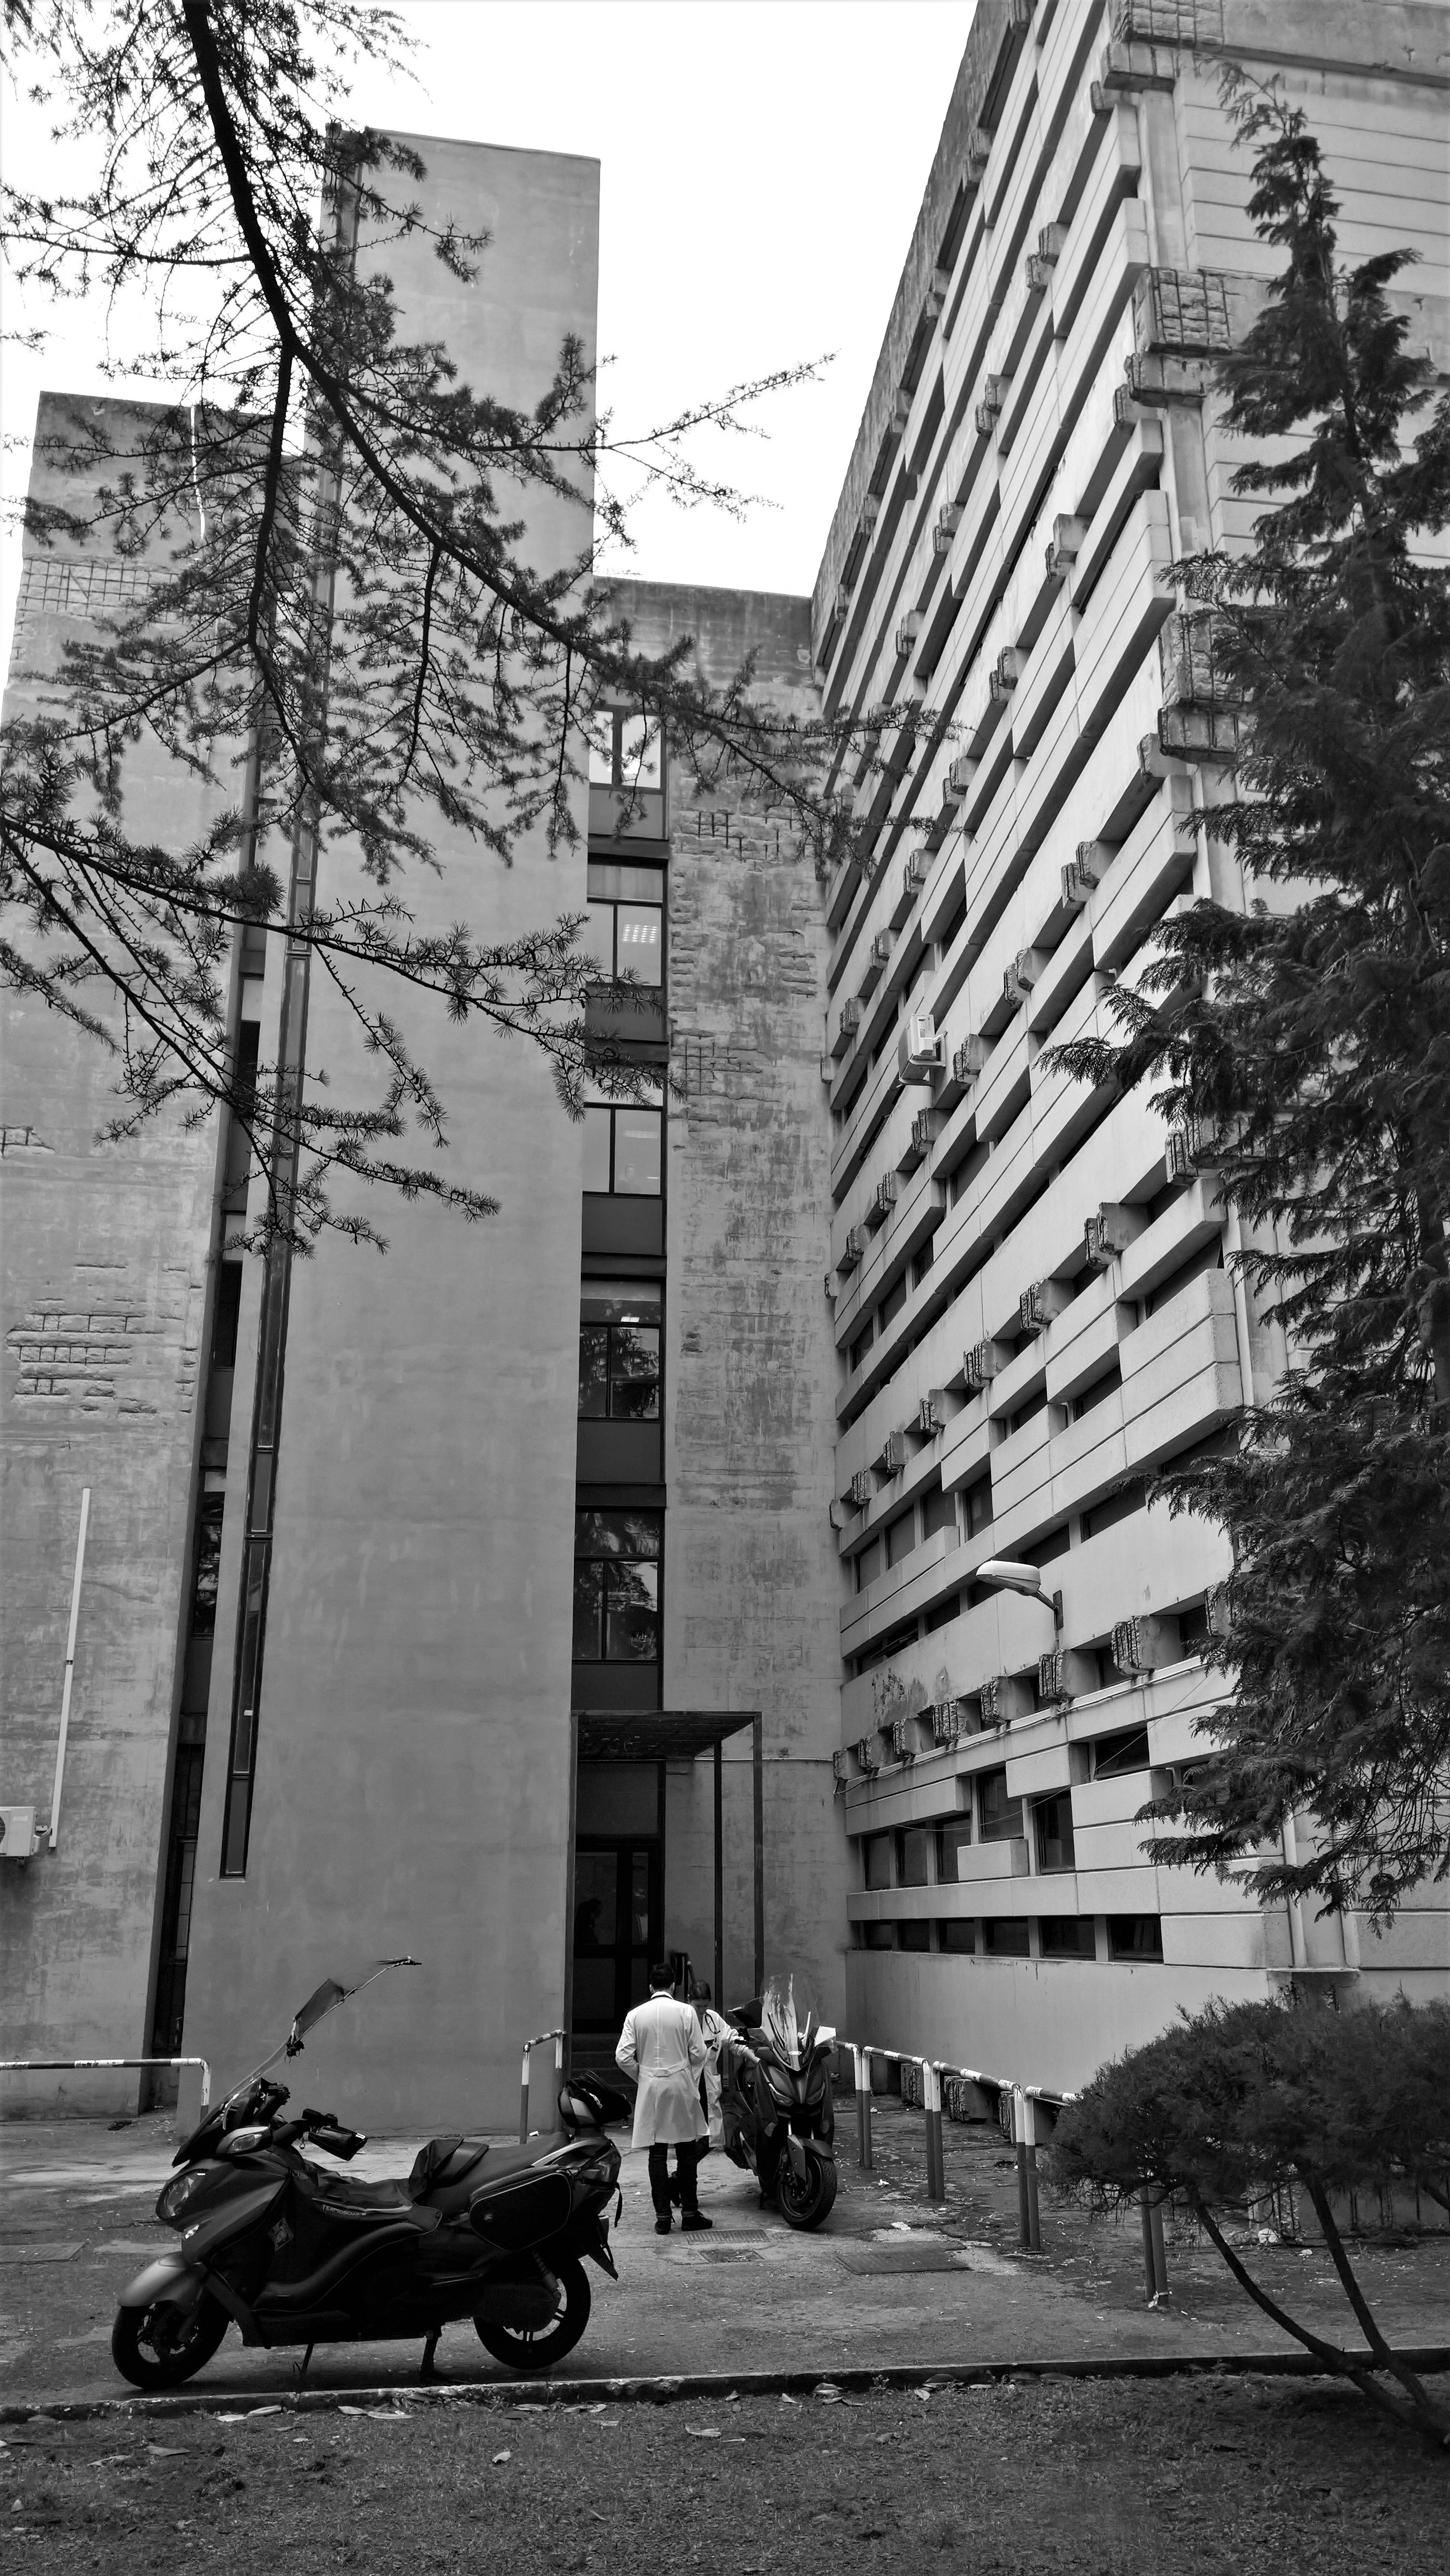
\includegraphics[height=0.4\textheight]{6_2_cap/img/ed22}}
	\caption{L'edificio 2. Particolari del Corpo A.}\label{esterno}
\end{figure}

Segue, quindi, la descrizione numerica dei componenti (opachi e trasparenti) utilizzati come dati di input per il calcolo del fabbisogno energetico e del carico termico (estivo e invernale) dell'edificio stesso.
\subsection{Componenti opachi}
\subsubsection{MURO EXT}
È il componente esterno verticale delle facciate maggiori del Corpo A. \\È caratterizzato esternamente da blocchi di silicalcite alternati dagli infissi. \\Questa tipologia di muro è fittizia poiché si è modellato un componente che nella realtà è caratterizzata da una diversa stratigrafia in senso verticale. Dal punto di vista numerico, quindi, si è effettuata una media ponderale delle varie caratteristiche termo-fisiche in modo tale che il risultato finale sia quanto più possibile veritiero. La parte inferiore è costituita semplicemente da un mattone forato da \n{10}{cm} intonacato internamente ed esternamente; la parte superiore, invece, è caratterizzata dai blocchi di silicalcite. \\ La stratigrafia della parte superiore è (dall'interno verso l'esterno):
\begin{center}
	\begin{tabular}{lcc}
		\toprule
		Componente & Spessore [m] & Conduttività [\si{W/mK}] \\
		\midrule
		Acciao & \num{0.01} & \num{50.0} \\
		Intercapedine d'aria & \num{0.05} & -\\
		CLS & \num{0.35} & \num{1.06} \\
		\bottomrule
	\end{tabular}
\end{center}
Questi i risultati del componente modellato (a valle della media ponderale):
\begin{center}
	\begin{tabular}{lcc}
		\toprule
		Spessore & \num{0.43} & \si{m}\\
		Trasmittanza & \num{1.423} & \trasm\\
		Trasmittanza termica periodica & \num{0.190} & \trasm\\
		\bottomrule
	\end{tabular}
\end{center}
\newpage
\subsubsection{MURO EXT 200}
È il componente esterno delle pareti in cemento armato.
\begin{center}
	\begin{tabular}{lcc}
		\toprule
		Componente & Spessore [m] & Conduttività [\si{W/mK}] \\
		\midrule
		Malta di calce-cemento & \num{0.01} & \num{0.90} \\
		CLS & \num{0.18} & \num{1.48}\\
		Malta di calce-cemento & \num{0.01} & \num{0.90} \\
		\bottomrule
	\end{tabular}
\end{center}
Questi i risultati del componente modellato:
\begin{center}
	\begin{tabular}{lcc}
		\toprule
		Spessore & \num{0.20} & \si{m}\\
		Trasmittanza & \num{3.29} & \trasm\\
		Trasmittanza termica periodica & \num{1.71} & \trasm\\
		\bottomrule
	\end{tabular}
\end{center}

\subsubsection{MURO EXT Corpo Basso}
È il componente esterno verticale dei corpi bassi ovvero B, C, D ed E.
\begin{center}
	\begin{tabular}{lcc}
		\toprule
		Componente & Spessore [m] & Conduttività [\si{W/mK}] \\
		\midrule
		Malta di calce-cemento & \num{0.01} & \num{0.90} \\
		Mattone forato & \num{0.08} & -\\
		Intercapedine d'aria & \num{0.05} & - \\
		CLS & \num{0.1} & \num{1.91}\\
		\bottomrule
	\end{tabular}
\end{center}
Questi i risultati del componente modellato:
\begin{center}
	\begin{tabular}{lcc}
		\toprule
		Spessore & \num{0.24} & \si{m}\\
		Trasmittanza & \num{1.63} & \trasm\\
		Trasmittanza termica periodica & \num{1.06} & \trasm\\
		\bottomrule
	\end{tabular}
\end{center}
\subsubsection{COPERTURA 1}
È la copertura del Corpo A.\\Già oggetto di interventi passati, le sue caratteristiche termo-fisiche sono così riassunte:
\begin{center}
	\begin{tabular}{lcc}
		\toprule
		Spessore & \num{0.38} & \si{m}\\
		Trasmittanza & \num{0.36} & \trasm\\
		Trasmittanza termica periodica & \num{0.10} & \trasm\\
		\bottomrule
	\end{tabular}
\end{center}
\subsubsection{COPERTURA 2}
È la copertura dei Corpi B, C, D ed E. In \vref{cap2} si può apprezzare l'elevato stato di usura dei prefabbricati costituenti la copertura dei corpi \emph{bassi}.
\begin{figure}[h]
	\centering
	\includegraphics[width=\textwidth]{6_2_cap/img/cop2}
	\caption[Veduta esterna del corpo E]{Veduta esterna del corpo E. Sullo sfondo il corpo C e A.}\label{cap2}
\end{figure}
\begin{center}
	\begin{tabular}{lcc}
		\toprule
		Componente & Spessore [m] & Conduttività [\si{W/mK}] \\
		\midrule
		Intonaco di Calce e Gesso & \num{0.02} & \num{1.61} \\
		CLS SC  & \num{0.09} & \num{1.48}\\
		CLS SA & \num{0.10} & \num{0.58} \\
		Bitume su carta e cartone & \num{0.0050} & \num{0.23} \\
		\bottomrule
	\end{tabular}
\end{center}
Questi i risultati del componente modellato:
\begin{center}
	\begin{tabular}{lcc}
		\toprule
		Spessore & \num{0.22} & \si{m}\\
		Trasmittanza & \num{2.39} & \trasm\\
		Trasmittanza termica periodica & \num{1.07} & \trasm\\
		\bottomrule
	\end{tabular}
\end{center}
\newpage
\subsubsection{PAVIMENTO}
È il componente opaco utilizzato per modellare il pavimento dell'Edificio 2 (quindi in comune a tutti i corpi). È bene precisare che questo componente non è a contatto con il terreno in quanto vi sono i locali della sottocentrale nel piano -1.\\
Questi i risultati:
\begin{center}
	\begin{tabular}{lcc}
		\toprule
		Componente & Spessore [m] & Conduttività [\si{W/mK}] \\
		\midrule
		Piastrelle di Ceramica & \num{0.01} & \num{1.30} \\
		CLS SC & \num{0.08} & \num{1.61}\\
		Blocco da solaio & \num{0.22} & - \\
		\bottomrule
	\end{tabular}
\end{center}
\begin{center}
	\begin{tabular}{lcc}
		\toprule
		Spessore & \num{0.31} & \si{m}\\
		Trasmittanza & \num{1.38} & \trasm\\
		Trasmittanza termica periodica & \num{0.35} & \trasm\\
		\bottomrule
	\end{tabular}
\end{center}
\clearpage
\subsection{Componenti trasparenti}
Come è già stato ampiamente detto, tutti gli infissi risultano essere ancora quelli originali.

Per la loro modellazione sono stati usati gli stessi dati termo-fisici ($U_g$, $U_f$ e $U_w$) mentre sono stati differenziati solo geometricamente.
Il telaio è metallico senza taglio termico con un unico vetro (spessore di \n{4}{mm} senza alcun trattamento superficiale).

Questi i risultati:
\begin{center}
	\begin{tabular}{lcc}
		\toprule
		$U_g$ & \num{5.747} & \multirow{3}*{\trasm}\\
		$U_f$ & \num{5.800} &\\
		$U_g$ & \num{5.760} &\\
		\bottomrule
	\end{tabular}
\end{center}

Si elencano ora i vari infissi utilizzati all'interno del modello dell'edificio:
\begin{itemize}
	\item \textbf{PICCOLA} \n{1.60x0.33}{m}.\\ È il componente trasparente facente parte delle facciate maggiori del Corpo~A. 
	\item \textbf{GRANDE} \n{1.60x0.67}{m}.\\ È la variante alta della finestra \textbf{PICCOLA}. 
	\item \textbf{LUCERNARIO} \n{1.45x0.39}{m}.\\ Questo è il lucernario presente nella parte superiore di ogni modulo delle due facciate maggiori del Corpo A. In \vref{unitloca} si possono vedere queste 3 tipologie di componenti trasparenti che caratterizzano le facciate maggiori del corpo A.
	\item \textbf{QUADRA} \n{0.75x0.75}{m}. Vedere \vref{finq}.
	\item \textbf{LUNGA} \n{0.75x1.70}{m}.\\ Presente al di sotto della finestra \textbf{QUADRA}, insieme a quest'ultima crea un unico infisso che percorre tutta l'altezza del Corpo A nelle scanalature del muro \textbf{MURO EXT 200}. 
	\item \textbf{FIN-160} \n{1.60x3.00}{m}. \\ Presente nel corridoio antistante la \emph{medicheria} in ogni piano. Anche questo infisso, come \textbf{FINESTRA LUNGA} e \textbf{FINESTRA QUADRA}, genera un'unica finestra che percorre tutta l'altezza del corpo A. In \vref{fin1} se ne può apprezzare un particolare.
	\item \textbf{PT-160} \n{1.60x2.00}{m}. \\ È la finestra dei Corpi B, C, D ed E. Vedere \vref{fincb}.
	\item \textbf{PT-Alta Corpo Basso} \n{1.60x0.35}{m}.\\ È il lucernario di ogni modulo caratterizzante i Corpi B, C, D ed E. 
\end{itemize}

\begin{figure}[t]
	\centering
	\includegraphics[width=\textwidth]{6_2_cap/img/fin1}
	\caption[Particolare del componente FIN-160]{Particolare del componente \textbf{FIN-160}: notare lo spessore di \n{4}{mm} della lastra di vetro.}\label{fin1}
\end{figure}

\begin{figure}[t]
	\centering
	\subfloat[][\emph{Una delle \textbf{PT-160} del corpo C. Sotto l'elemento di cemento armato ad U capovolto è presente \textbf{PT-Alta Corpo Basso}.}]{\includegraphics[width=0.35\textwidth]{6_2_cap/img/fincb}\label{fincb}} \quad
	\subfloat[][\emph{Due finestre \textbf{QUADRA}.}]{\includegraphics[width=0.35\textwidth]{6_2_cap/img/finq}\label{finq}} 
	\caption{Alcuni componenti trasparenti dell'edificio 2.}
\end{figure}

A conclusione dell'analisi si evidenzia come tutti i valori di trasmittanza calcolati sia per le strutture opache verticali che quelle orizzontali come anche i componenti trasparenti risultano sensibilmente superiori ai valori limite contenuti nel DM 26/6/2015.

\subsection{Definizione locali}
Il carico termico di un edificio (come anche il suo fabbisogno energetico) non tiene conto solamente dell'ambiente esterno (temperatura e umidità tutto l'anno mentre la radiazione solare solo in estate). È molto importante considerare la destinazione d'uso del locale che si intende climatizzare. Pertanto sono stati individuati le tipologie di locali e per ognuno di essi si sono definiti i seguenti parametri:
\begin{itemize}
	\item \emph{Temperatura} e \emph{umidità relativa} di progetto nella stagione estiva e invernale. Una loro adeguata scelta in fase progettuale e poi un loro mantenimento ad impianto ultimato e perfettamente funzionante sono alla base del benessere di una persona che vive in un locale;
	\item La \emph{portata di rinnovo} dalla norma \norvent. Rappresenta la quantità di aria esterna che si suppone essere priva di agenti nocivi per l'uomo e che è necessario introdurre all'interno dell'ambiente da climatizzare per mantenere entro certi limiti la qualità, appunto, dell'aria;
	\item Gli \emph{apporti interni di calore}:
	\begin{itemize}
		\item \emph{L'occupazione}, ovvero il numero di persone che affollano il locale con i conseguenti apporti di calore sensibile e latente. In assenza di dati certi (ovvero nell'impossibilità di conoscere le persone che effettivamente affollano un locale - contando il numero di posti a sedere in una sala di un cinema, per esempio) si procede utilizzando i valori di occupazione fissati dalla \norvent;
		\item \emph{Apparati interni}, ovvero i carichi dovuti a macchinari/fonti di calore sensibile e latente presenti all'interno del locale;
		\item \emph{L'illuminazione}, ovvero la quantità di calore sensibile (trasmesso per convezione e irraggiamento) dovuto all'illuminazione;
	\end{itemize}
\end{itemize}
È molto importante notare che per alcuni di questi apporti interni di calore sono stati definiti dei profili d'uso temporali su base oraria. \emph{L'occupazione} dello Studio Medico, per esempio, ha un profilo d'uso del tipo:
\begin{center}
	\begin{tabular}{lr}
		\toprule
		Dalle 00:00 alle 08:00 & 0\% \\
		Dalle 08:00 alle 17:00 & 100\% \\
		Dalle 17:00 alle 00:00 & 0\% \\
		\bottomrule
	\end{tabular}
\end{center}
Ovvero all'interno degli studi medici vi sarà il massimo dell'occupazione (calcolata considerando l'indice di affollamento $n_S$ che in questo caso è pari a \n{0.05}{pers/m^2} tratto sempre dalla \norvent) dalle 8:00 alle 17:00 ogni giorno dell'anno.

Un ulteriore aspetto da considerare è l'illuminazione dei locali a destinazione d'uso sanitaria. La maggior parte dei corpi illuminanti consiste in \emph{lampade a fluorescenza} avente efficienza luminosa di circa \n{80}{lm/W}. Dopo aver verificato la potenza effettivamente installata e note le superfici è stato possibile ricavare un indicatore in \si{W/m^2} per ogni locale. Qui di seguito i risultati utilizzati come dati di input:
\begin{itemize}
	\item \n{10}{W/m^2} negli uffici, studi medici, segreteria;
	\item \n{19}{W/m^2} negli ambulatori, laboratori, sale operatorie e degenza;
	\item \n{10}{W/m^2} nei corridoi, atri e sale d'attesa;
	\item \n{9}{W/m^2} nei depositi e magazzini;
	\item \n{8}{W/m^2} nei bagni, spogliatoi e lavatoi.
\end{itemize}

Si vogliono descrivere in maniera dettagliata alcune tipologie di locali che sono stati maggiormente utilizzati per la modellazione dell'edificio.

\newpage
\subsubsection{Degenza}
\begin{figure}[h]
	\centering
	\includegraphics[height=0.5\textwidth]{6_2_cap/img/deg}
	\caption{Posizione delle degenze all'interno del corpo A.}\label{deg}
\end{figure}
\begin{center}
	\begin{tabular}{lcc}
										& Raffrescamento 			& Riscaldamento \\
		Temperatura interna di progetto & \n{24.0}{\degreeCelsius} 	& \n{21.0}{\degreeCelsius}\\
		Umidità interna di progetto 	& \n{50.0}{\%}				& \n{30.0}{\%}\\
		\midrule
		Ventilazione					& \multicolumn{2}{c}{\n{11}{l/s} per persona} 		\\
		\midrule
		\multirow{3}*{Occupazione}		& \multicolumn{2}{c}{\n{5}{m^2/pers}}  		\\
									 	& \n{75}{W/pers} 		& sensibile	\\
										& \n{70}{W/pers}		& latente 	\\
		\midrule
		Apparati interni 				&\n{15}{W/m^2}			& sensibile\\
		\midrule
		Illuminazione					& \multicolumn{2}{c}{\n{19}{W/m^2}}\\
		\midrule
		Altri carichi					& \multicolumn{2}{c}{--}\\				
	\end{tabular}
\end{center}

\newpage
\subsubsection{Laboratorio}
\begin{figure}[h]
	\centering
	\includegraphics[height=0.5\textwidth]{6_2_cap/img/lab}
	\caption{Posizione dei laboratori nei corpi A e C.}\label{lab}
\end{figure}
\begin{center}
	\begin{tabular}{lcc}
										& Raffrescamento 			& Riscaldamento \\
		Temperatura interna di progetto & \n{25.0}{\degreeCelsius} 	& \n{21.0}{\degreeCelsius}\\
		Umidità interna di progetto 	& \n{50.0}{\%}				& \n{50.0}{\%}\\
		\midrule
		Ventilazione					& \multicolumn{2}{c}{\n{6}{vol/h}} 		\\
		\midrule
		\multirow{3}*{Occupazione}		& \multicolumn{2}{c}{\n{20}{m^2/pers}}  		\\
										& \n{75}{W/pers} 		& sensibile	\\
										& \n{55}{W/pers}		& latente 	\\
		\midrule
		Apparati interni 				&\n{40}{W/m^2}			& sensibile\\
		\midrule
		Illuminazione					& \multicolumn{2}{c}{\n{19}{W/m^2}}\\
		\midrule
		Altri carichi					& \n{1000}{W}			& sensibile \\				
	\end{tabular}
\end{center}

\newpage
\subsubsection{Studio Medico}
\begin{figure}[h]
	\centering
	\includegraphics[height=0.5\textwidth]{6_2_cap/img/stm}
	\caption{Posizione degli studi medici nei corpi A e C.}\label{stm}
\end{figure}
\begin{center}
	\begin{tabular}{lcc}
										& Raffrescamento 			& Riscaldamento \\
		Temperatura interna di progetto & \n{25.0}{\degreeCelsius} 	& \n{22.0}{\degreeCelsius}\\
		Umidità interna di progetto 	& \n{50.0}{\%}				& \n{40.0}{\%}\\
		\midrule
		Ventilazione					& \multicolumn{2}{c}{\n{11}{l/s} per persona} 		\\
		\midrule
		\multirow{3}*{Occupazione}		& \multicolumn{2}{c}{\n{4}{pers}}  		\\
										& \n{75}{W/pers} 		& sensibile	\\
										& \n{55}{W/pers}		& latente 	\\
		\midrule
		Apparati interni 				&\multicolumn{2}{c}{--}\\
		\midrule
		Illuminazione					& \multicolumn{2}{c}{\n{10}{W/m^2}}\\
		\midrule
		Altri carichi					& \multicolumn{2}{c}{--}\\				
	\end{tabular}
\end{center}

\newpage
\subsubsection{Cucina}
\begin{figure}[h]
	\centering
	\includegraphics[height=0.5\textwidth]{6_2_cap/img/cuc}
	\caption{Posizione delle cucine nei corpi A e C.}\label{cuc}
\end{figure}
\begin{center}
	\begin{tabular}{lcc}
										& Raffrescamento 			& Riscaldamento \\
		Temperatura interna di progetto & \n{28.0}{\degreeCelsius} 	& \n{20.0}{\degreeCelsius}\\
		Umidità interna di progetto 	& \n{50.0}{\%}				& \n{30.0}{\%}\\
		\midrule
		Ventilazione					& \multicolumn{2}{c}{\n{16.5}{l/s} per \si{m^2}} 		\\
		\midrule
		\multirow{3}*{Occupazione}		& \multicolumn{2}{c}{\n{5}{m^2/pers}}  		\\
										& \n{75}{W/pers} 		& sensibile	\\
										& \n{70}{W/pers}		& latente 	\\
		\midrule
		Apparati interni 				& \n{5.40}{W/m^2} 		& sensibile \\
		\midrule
		Illuminazione					& \multicolumn{2}{c}{\n{10}{W/m^2}}\\
		\midrule
		\multirow{2}{*}{Altri carichi}	& \n{1500}{W} 		& sensibile \\
										& \n{500}{W} 		& latente   \\
	\end{tabular}
\end{center}

\newpage
\subsubsection{Ufficio}
\begin{figure}[h]
	\centering
	\includegraphics[height=0.5\textwidth]{6_2_cap/img/lab}
	\caption{Posizione degli uffici nei corpi A e C.}\label{uff}
\end{figure}
\begin{center}
	\begin{tabular}{lcc}
										& Raffrescamento 			& Riscaldamento \\
		Temperatura interna di progetto & \n{25.0}{\degreeCelsius} 	& \n{21.0}{\degreeCelsius}\\
		Umidità interna di progetto 	& \n{50.0}{\%}				& \n{40.0}{\%}\\
		\midrule
		Ventilazione					& \multicolumn{2}{c}{\n{11}{l/s} per persona} 		\\
		\midrule
		\multirow{3}*{Occupazione}		& \multicolumn{2}{c}{\n{10}{m^2/pers}}  		\\
										& \n{75}{W/pers} 		& sensibile	\\
										& \n{70}{W/pers}		& latente 	\\
		\midrule
		Apparati interni 				& \n{15}{W/m^2} 		& sensibile \\
		\midrule
		Illuminazione					& \multicolumn{2}{c}{\n{10}{W/m^2}}\\
		\midrule
		Altri carichi					& \multicolumn{2}{c}{--}\\
	\end{tabular}
\end{center}

\newpage
\section{L'impianto}
L'impianto dell'Edificio 2 è attualmente caratterizzato da una sottocentrale, presente nel piano \num{-1}, la quale alimenta varie unità locali (radiatori e fancoil) e UTA oltre a produrre (tramite due bollitori da \n{5000}{l} ciascuno) acqua calda sanitaria.

Nel primo capitolo è già stato ampiamente detto che i vari edifici del Policlinico sfruttano la rete di presidio di acqua surriscaldata e refrigerata.

Partendo dal lato utenza, il carico sensibile invernale viene coperto da radiatori (si veda la \subref{radiatori} in \vref{unitloca}) presenti all'interno di ogni piano e fancoil solo nel III e IV piano. Il carico estivo (sia sensibile che latente) invece viene coperto da monosplit e fancoil ad acqua montati negli ultimi anni durante varie ristrutturazioni (come nel caso del terzo e quarto piano). In questi due piani vi è anche una rete aeraulica per il rinnovo dell'aria. Nonostante la presenza di questi impianti, non vengono garantiti l'adeguato recupero energetico dall'impianto di ventilazione e il controllo termo-igrometrico dai fancoil e radiatori. Queste carenze sono evidenti nell'eccessivo ricorso a split per il controllo della temperatura (e in modo indiretto dell'umidità) durante la stagione estiva. È evidente la necessità di una riqualificazione. Negli altri 3 piani la ventilazione è garantita tramite infiltrazione naturale (ovvero apertura delle finestre di piano) mentre è assente del tutto il controllo termo-igrometrico nella stagione estiva. Anche in questi piani si è fatto largo uso di monosplit a parete.

\begin{figure}[h!]
	\centering
	\subfloat[][\emph{Un tipico radiatore presente nel corridoio del Piano Terra -- Corpo A.}]{\includegraphics[width=0.45\textwidth]{6_2_cap/img/radiatore}\label{radiatori}}	\quad
	\subfloat[][\emph{Corridoio del IV Piano. Si noti il mix di unità locali.}]{\includegraphics[width=0.45\textwidth]{6_2_cap/img/P4RadFan}}	\\
	\subfloat[][\emph{Area Relax del IV Piano. In alto la griglia di mandata del fancoil. Questi hanno anche una presa di aria di rinnovo esterna.}]{\includegraphics[width=0.45\textwidth]{6_2_cap/img/P4FanCoil}} \quad
	\subfloat[][\emph{Diffusore circolare in una degenza del III Piano per l'aria di rinnovo.}]{\includegraphics[width=0.45\textwidth]{6_2_cap/img/P3Aer}}
	\caption{Unità Locali nel Corpo A}\label{unitloca}
\end{figure}
	
Il quinto piano (in cui è presente il blocco operatorio di cardiochirurgia) è gestito da un adeguato impianto a tutt'aria presente in copertura.

In una porzione del primo piano vi è l'UTIC (\emph{Unità di Terapia Intensiva Coronarica}) che è trattata da un altro impianto a tutt'aria montato in un locale dello stesso piano. L'UTA dell'Emodinamica (al Piano Terra) con la relativa centrale termo-frigorifera è presente all'esterno.

Nonostante siano state elencati e descritti gli usi dei diversi edifici, l'intervento di riqualificazione energetica riguarda solo i corpi C e A. Di quest'ultimo edificio è escluso \emph{in toto} il blocco operatorio presente al quinto piano mentre dell'UTIC e dell'Emodinamica verrà effettuato solo un intervento civile (ovvero non verrà intaccato l'impianto aeraulico).

In \vref{img:PT}, \vref{img:P1}, \vref{img:P2}, \vref{img:P3} e \vref{img:P4} si riportano le planimetrie con le aree di intervento dei singoli piani.

%\includepdf[pagecommand={\null\vfill\captionof{table}{caioooo}}]{6_2_cap/img/PT.pdf}\label{PT}
\begin{sidewaysfigure}
	\centering
		\includegraphics[width=\hsize]{6_2_cap/img/PT}
		\caption{Planimetria Piano Terra -- Edificio 2}
		\label{img:PT}
\end{sidewaysfigure}
\begin{sidewaysfigure}
	\centering
		\includegraphics[width=\hsize]{6_2_cap/img/P1}
			\caption{Planimetria Piano Primo -- Corpo A}
			\label{img:P1}
\end{sidewaysfigure}
\begin{sidewaysfigure}
	\centering
	\includegraphics[width=\hsize]{6_2_cap/img/P2}
	\caption{Planimetria Piano Secondo -- Corpo A}
	\label{img:P2}
\end{sidewaysfigure}
\begin{sidewaysfigure}
	\centering
	\includegraphics[width=\hsize]{6_2_cap/img/P3}
	\caption{Planimetria Piano Terzo -- Corpo A}
	\label{img:P3}
\end{sidewaysfigure}
\begin{sidewaysfigure}
	\centering
	\includegraphics[width=\hsize]{6_2_cap/img/P4}
	\caption{Planimetria Piano Quarto -- Corpo A}
	\label{img:P4}
\end{sidewaysfigure}

%\includepdf{6_2_cap/img/PT.pdf}\label{PT}
%\includepdf{6_2_cap/img/P1.pdf}\label{P1}
%\includepdf{6_2_cap/img/P2.pdf}\label{P2}
%\includepdf{6_2_cap/img/P3.pdf}\label{P3}
%\includepdf{6_2_cap/img/P4.pdf}\label{P4}
\clearpage
\section{I risultati energetici}
\begin{figure}[p]
	\centering
	\subfloat[][Radiatori]{\includegraphics[width=0.45\textwidth]{6_2_cap/img/rad}\label{rad}}\quad
	\subfloat[][V Piano]{\includegraphics[width=0.45\textwidth]{6_2_cap/img/vpiano}\label{vpiano}}\\
	\subfloat[][Emodinamica]{\includegraphics[width=0.45\textwidth]{6_2_cap/img/emo}\label{emo}}\quad
	\subfloat[][UTIC]{\includegraphics[width=0.45\textwidth]{6_2_cap/img/utic}\label{utic}}\\
	\subfloat[][Corpo A]{\includegraphics[width=0.45\textwidth]{6_2_cap/img/ca}\label{ca}}\quad
	\subfloat[][Corpo C]{\includegraphics[width=0.45\textwidth]{6_2_cap/img/cb}\label{cb}}
	\caption{Le zone termiche}\label{zt}
\end{figure}

L'edificio è stato suddiviso in 5 zone termiche visualizzabili in \vref{zt}:
\begin{itemize}
	\item \textbf{V Piano};
	\item \textbf{UTIC};
	\item \textbf{Emodinamica};
	\item \textbf{Corpo A} (escluse le zone del V Piano, UTIC e Emodinamica);
	\item \textbf{Corpo C};
	\item \textbf{Radiatori}: ovvero tutti i servizi igienici del Corpo A. 
\end{itemize}
È necessario spiegare il motivo di questa suddivisione.

Innanzitutto le prime tre zone termiche sono state separate dal resto del Corpo A in quanto il loro impianto non è oggetto di intervento ma è comunque interessante conoscere il risparmio in potenza che si riesce ad ottenere modificando l'involucro.

Per quanto riguarda la zona \emph{Radiatori}, è effettivamente sbagliato dal punto di vista termico considerarla esclusa dal resto del Corpo A in quanto non sono due zone termiche distinte. Questa forzatura è stata necessaria in quanto dai risultati ottenuti non era possibile scindere i carichi sensibili dei servizi igienici dal resto dell'edificio. Siccome i radiatori verranno posizionati solo nei servizi igienici, era interessante conoscere, quindi, il carico termico dei soli servizi igienici per poi dimensionare adeguatamente l'impianto a suo servizio. 

\subsection{Stagione Estiva}
Si presentano i vari risultati ottenuti con la dovuta teoria che vi è alla base.

Nel secondo capitolo si è già abbondantemente spiegato il motivo per cui è necessario considerare anche i carichi interni e quelli latenti.

Le valutazioni energetiche sono state effettuate con una temperatura e umidità esterna rispettivamente di \n{35}{\degreeCelsius} con il \n{60}{\%} maggiore di quella consigliata dalla \norvent\ per la città di Napoli. All'interno, invece, si sono rispettate le condizioni di benessere termo-igrometrico: \n{24}{\degreeCelsius} con il \n{50}{\%}. Per la ventilazione si è proceduto considerando per ogni locale i ricambi orari minimi.

Relativamente ai soli reparti di Emodinamica, UTIC e Blocco Operatorio che possiedono un loro impianto dedicato a \emph{tutt'aria} si è proceduto in questo modo:
sono note le superfici e le altezze dei vari locali come anche il carico esterno solare e di trasmissione; si sono supposti i \num{10} ricambi orari di aria esterna (per le sale chirurgiche e di terapia intensiva del blocco operatorio si sono fissati i \num{20} ricambi orari arrivando a \num{11} ricambi medi su tutto il piano); un affollamento di $n=\SI{0.08}{pers/m^2}$; un carico sensibile e latente per le persone pari rispettivamente a $Q_{\mathrm{pers,S}}=\SI{70}{W/pers}$ e $Q_{\mathrm{pers,L}}=\SI{50}{W/pers}$; un carico interno per le varie apparecchiature di $Q_{\mathrm{int,S}}=\SI{10}{W/m^2}$. 

Nella seguente tabella sono mostrati i parametri di input e i risultati per le 3 zone termiche considerate.
\begin{center}
	\begin{tabular}{lccccc}
		\toprule
					&	Superficie 				&	Portata Aria Est. 			&	$\dot{Q}_{\mathrm{sol}}+\dot{Q}_{\mathrm{trasm}}$		& 	\multirow{2}{*}{RST}		&	$\dot{Q}_{\mathrm{frigo}}$ 	\\
					&	{\small \si{m^2}}		&		{\small \si{kg/s}}		&		{\small \si{kW}}				&								&{\small \si{kW}}		\\					
		\midrule	
		UTIC		&		\num{146}			&		\num{1.46}				&	\num{7.62}		&	0.94					&	\num{10.5}		\\
		Emod.		&		\num{169}			&		\num{1.69}				&	\num{13.2}		&	0.96					&	\num{16.5}		\\
		B.O.		&	\num{697}				&		\num{7.33}				&	\num{34.6}		&	0.94					&	\num{48.3}		\\
		\bottomrule
	\end{tabular}
\end{center}
RST sta per \emph{Rapporto Sensibile su Totale} ed è adimensionale. È molto importante nei diagrammi psicrometrici in quanto permette di individuare i luoghi dei punti di immissione dell'aria (nel caso di impianti a tutt'aria o di miscelazione in quelli misti) che bilanciano adeguatamente sia il carico sensibile che latente. Siccome nel nostro caso il suo valore è prossimo all'unità avremo un carico da bilanciare che è pressoché tutto sensibile.

Conoscendo il valore di RST, del carico da bilanciare $Q_{frigo}$ e della portata di ventilazione, dal diagramma psicrometrico si individuano, per ogni zona termica (e le loro rispettive UTA), le proprietà termoigrometriche dell'aria da immettere. Ed è, quindi, possibile calcolare le potenze delle batterie di raffreddamento e post-riscaldamento delle UTA nel caso estivo. Nella seguente tabella sono riassunti i risultati ottenuti in \si{kW}. L'ipotesi alla base di tutte queste valutazioni è che le batterie siano ideali cioè che non vi sia una frazione di portata d'aria che non entri a contatto con le lamelle delle batterie stesse. In questa sede, però, volendo solo effettuare una valutazione pre e post intervento non è importante considerare anche il cosiddetto \emph{by-pass factor} delle batterie (anche se oggigiorno suddetti fattori risultano essere dell'ordine del \n{5}{\%} e quindi tranquillamente trascurabili).
\begin{center}
	\begin{tabular}{lcc}
		&	$\dot{Q}_{\mathrm{UTA,f}}$		&	$\dot{Q}_{\mathrm{UTA,c}}$\\
		\midrule
		UTIC	&	\num{79.3}			&	\num{6.86}\\
		Emod.	&	\num{91.7}			&	\num{3.52}\\
		B.O.	&	\num{664}			&	\num{39.0}\\
	\end{tabular}
\end{center}
La potenza di raffreddamento e riscaldamento viene fornita da una opportuna portata d'acqua prodotta in sottocentrale. Una rapida valutazione delle portate in gioco, restituisce i valori, in \si{l/s}, riportati nella tabella successiva. Per questioni tecnologiche le temperature di mandata e ritorno dell'acqua sono rispettivamente di \num{7} e \n{12}{\degreeCelsius} per la batteria di raffreddamento mentre di \num{60} e \n{55}{\degreeCelsius} per quelle di riscaldamento e che il calore specifico dell'acqua è ritenuto costante e pari a $c_p=\SI{4.2}{kJ/kgK}$.
\begin{center}
	\begin{tabular}{lcc}
			&	$\dot{m}_f$	&	$\dot{m}_c$\\
			\midrule
			UTIC	&	\num{3.8}	&	\num{0.33}\\
			Emod.	&	\num{4.4}	&	\num{0.17}\\
			B.O.	&	\num{32}		&	\num{1.8}\\
	\end{tabular}
\end{center}

Per quanto riguarda \corpa\ e \corpc, l'impianto utilizzato è di tipo \emph{misto} (come nel III e IV piano) o addirittura assente. Pertanto non ne è stata effettuata una valutazione sulla ventilazione ma i risultati considerano solo la trasmissione tramite l'involucro e i carichi interni: apparecchiature e persone.

Per la zona termica \radd\ è ovvio che il carico di raffreddamento sia nullo.

In \vref{stato:fatto} sono riassunti tutti i risultati ottenuti per la stagione estiva nello stato di fatto. 
%{Per i radiatori ovviamente la potenza di raffrescamento è nulla. Per UTIC, BO e EMO il totale tiene conto della trasmissione (ottenuta da CYPE) mentre i carichi interni (sensibili e latenti) sono stati calcolati su Excel. Poi tramite diagramma psicrometrico ho calcolato anche la potenza di ventilazione. Per i corpi A e C i valori del sensibile e del latente non tengono conto della ventilazione.}
\begin{table}
		\centering
		\small
		\begin{tabular}{lccccc}
			\toprule
			\multirow{2}*{Zona Termica} & Superficie 		& Ventilazione 					& $\dot{Q}_L$ 			& $\dot{Q}_S$ 					& $\dot{Q}_{\mathrm{frigo}}$  \\
			& \si{m^2}		& \si{m^3/h}						& \si{kW}			& \si{kW}					& \si{kW}\\
			\midrule
			Radiatori		& \num{291.1}				& ---								& ---				& ---						& ---\\
			B.O.			& \num{696.7}				& \num{21936}						& \num{2.78}		& \num{45.5}				& \num{447.3}\\
			UTIC			& \num{145.7}				& \num{4371}						& \num{0.583}		& \num{9.89}				& \num{89.7}\\
			Emod.			& \num{164.4}				& \num{5058}						& \num{0.674}		& \num{15.9} 				& \num{108.2}\\
			Corpo C			& \num{529.2}				& --								& \num{2.3}			& \num{81.7}				& \num{84}\\
			Corpo A			& \num{2352.2}				& --								& \num{20.6}		& \num{212}					& \num{233}\\
			\bottomrule
		\end{tabular}
	\caption{Carichi Termici estivi - Stato di fatto}\label{stato:fatto}
\end{table}

Si ricordi che i carichi sensibili e latenti per la stagione estiva sono definiti come segue:
\begin{align}
	\dot{Q}_S	&=\dot{Q}_{\mathrm{sol}}+\dot{Q}_{\mathrm{trasm}}+\dot{Q}_{\mathrm{int,S}}+\dot{Q}_{\mathrm{pers,S}}\\
	\dot{Q}_L	&=\dot{Q}_{\mathrm{int,L}}+\dot{Q}_{\mathrm{pers,L}}
\end{align}
\subsection{Stagione Invernale}
Come è già stato detto nel secondo capitolo, in questa stagione si trascura qualsiasi apporto di carico latente. Le valutazioni sono state fatte con una temperatura esterna di \n{0}{\degreeCelsius} mentre all'interno vengono garantiti i \n{22}{\degreeCelsius} col \n{45}{\%} di umidità relativa.

Per determinare le condizioni termoigrometriche di immissione dell'aria nell'UTIC, Emodinamica e nel Blocco Operatorio si è proceduto facendo un bilancio di energia:
\begin{align}
\dot{m}h_s	&	=\dot{m}h_i+\dot{Q}_{\mathrm{trasm}}		\label{bilancio}\\
h_s			&	=h_i+\frac{\dot{Q}_{\mathrm{trasm}}}{\dot{m}}	\notag\\
t_s			&	=\frac{t_ic_p\dot{m}+\dot{Q}_{\mathrm{trasm}}}{c_p\dot{m}}\label{bilancio2}
\end{align}
Nell'equazione \vref{bilancio2} si è supposta l'aria secca trascurando, quindi, il contributo del vapore d'acqua.

Con l'ausilio del diagramma psicrometrico, si è proceduto a valutare la potenza necessaria per abbattere il carico invernale. Sono note queste quantità: la portata di ventilazione (che si suppone uguale a quella estiva), il carico invernale da abbattere $\dot{Q}_{trasm}$, le condizioni interne e esterne, il valore di RST. Intersecando le varie rette corrispondenti alle altrettante trasformazioni si sono ottenuti i risultati ricercati riassunti nella seguente tabella. Ovviamente la potenza termica risultante $\dot{Q}_{vent}$ è la somma di quella necessaria alla batteria di pre e post riscaldamento.
\begin{center}
	\label{UTA:potenzaFATTO}
	\begin{tabular}{lcccc}
						& \multirow{2}{*}{RST}	&	$t_s$ 					& $\dot{Q}_{\mathrm{trasm}}$	&	$\dot{Q}_{\mathrm{vent}}$	\\
						&						&	\si{\degreeCelsius} &	\si{kW}				&	\si{kW}\\
		\midrule
		UTIC			&\multirow{3}{*}{1.1}	&	\num{25.3}		&\num{4.75}				&	\num{55.4}\\
		Emod.			&						&	\num{29.4}		&\num{12.5}				&	\num{70.8}\\
		B.O.			&						&	\num{27.2}		&\num{38.4}				&	\num{293}\\
	\end{tabular}
\end{center}
In definitiva, i risultati sono riportati di seguito per ogni zona termica. Anche in questo caso, per i corpi A e C non si è tenuto conto della ventilazione. In \vref{car:fatt} i risultati.
%{Per i Radiatori il totale tiene conto solo della trasmissione. Per BO, UTIC e EMO ho fatto la somma tra la trasmissione e la potenza di ventilazione calcolata tramite diagramma psicrometrico e ma i risultati stanno anche sul file excel. Per i due Corpi A e C il totale è solo la trasmissione in quanto non è presente la ventilazione.}
\begin{table}
	\centering
	\small
	\begin{tabular}{lcccc}
		\toprule
		\multirow{2}*{Zona Termica} & Superficie 		& Ventilazione 					& $\dot{Q}_{\mathrm{trasm}}$ 	 			& $\dot{Q}_{\mathrm{risc}}$		\\
									& \si{m^2}			& \si{m^3/h}					& \si{kW}					& \si{kW}		\\
		\midrule
		Radiatori					& \num{291.1}		& ---							& \num{30.7}				& \num{30.7}	\\
		B.O.						& \num{696.7}		& \num{21936}					& \num{38.4}				& \num{332}	\\
		UTIC						& \num{145.7}		& \num{4371}					& \num{4.75}				& \num{60.1}	\\
		Emod.						& \num{164.4}		& \num{5058}					& \num{12.5}				& \num{83.3} 	\\
		Corpo C						& \num{529.2}		& --							& \num{59.9}				& \num{59.9}	\\
		Corpo A						& \num{2352.2}		& --							& \num{142}					& \num{142}	\\
		\bottomrule
	\end{tabular}
	\caption{Carichi Termici invernali - Stato di fatto}\label{car:fatt}
\end{table}

La potenza totale tiene conto sia della trasmissione che della ventilazione calcolata nella tabella precedente.